\documentclass{beamer}

\usepackage{subfigure}
\usepackage{graphicx}
\usepackage{sidecap}
\usepackage{caption}
%\usepackage{subcaption}
\captionsetup{compatibility=false}
\usepackage{appendixnumberbeamer}
\usepackage{amsmath}
% --
\usepackage{multirow}
\usepackage{xcolor}
\usepackage{setspace}
\usepackage{hyperref}
\usepackage{anyfontsize}

\beamertemplatenavigationsymbolsempty
\setbeamertemplate{footline}

\newenvironment{itemise} {\begin{itemize} \setlength{\itemsep}{0.2cm}} {\end{itemize}}
\usepackage[labelformat=empty]{caption}
\setbeamertemplate{sections/subsections in toc}[square]

%% COLORS
\definecolor{Gray}{gray}{0.9}
\definecolor{dblue}{rgb}{0.132,0.1,0.27}
\definecolor{mint}{cmyk}{1.0, 0.2, 0.6, 0.05}
\definecolor{ant}{cmyk}{0.5, 0.1, 0.0, 0.45}
\definecolor{lgray}{cmyk}{0.12, 0.0, 0.0, 0.17}
\definecolor{lred}{cmyk}{0.0, 0.9, 0.7, 0.0}


\usepackage{etoolbox}% http://ctan.org/pkg/etoolbox 
\usepackage{booktabs}

\newenvironment{literatur}{%
  \parskip2pt \parindent0pt \raggedright
  \def\lititem{\hangindent=0.5cm \hangafter1}}{%
  \par\ignorespaces}

\newcommand{\tb}[1]{{\color{blue}{\textbf{#1}}}}
\newcommand{\tm}[1]{{\color{mint}{\textbf{#1}}}}
\newcommand{\tr}[1]{{\color{red}{\textbf{#1}}}}
% Ilya: packages

\usepackage{tikz}
\usepackage{lmodern}
\usepackage{enumitem}

% Ilya: my commands

\newenvironment{mytemize}
{\vfill\itemize[nolistsep,itemsep=\fill,label=\color{blue}{$\triangleright$}]}
  {\enditemize}


\newenvironment{mynumerate}
{\vfill\enumerate[nolistsep,itemsep=\fill,label=\arabic*.]}
  {\endenumerate}

\newcommand{\hitem}[1]{
  {\color{blue}{$\triangleright$}} 
  {#1} 
  {\hfill}
}

\setlist[itemize]{label= \color{blue}{$\triangleright$}}
\setlist[enumerate]{label = \arabic*.}

\newcommand{\rarr}{$\Rightarrow$\ }



%\href{<Ziel>}{<Eingefasster Text>} 

%\logo{\includegraphics[height=0.7cm]{BdFlogo.eps}\hspace{300pt}\vspace{-5pt}}
%\logo{\includegraphics[height=0.8cm]{BdFlogo.eps}}
%\logo{\pgfputat{\pgfxy(-6.2,-0.5)}{\pgfbox[center,base]{\includegraphics[height=0.8cm]{BdFlogo.eps}}}}

%------------------------------------------------------------------------------------
% TITLE
%------------------------------------------------------------------------------------
\title[PSME]{Macroeconomics\\ Lecture 4 -- Consumption, Savings and Balance of Payments} 
\author[I. Eryzhenskiy]{Ilya Eryzhenskiy}
\institute[BdF]{PSME Panth\'{e}on-Sorbonne Master in Economics}
\date[PSME macro]{Fall 2023}

%---BEGIN------------------------------------------------------------------------------
\begin{document}

\begin{frame}
  \maketitle
\end{frame}

\begin{frame}{Overview}
  \tableofcontents
\end{frame}


%---FRAME------------------------------------------------------------------------------
\section{2-period Consumer Problem}
%---FRAME------------------------------------------------------------------------------
\begin{frame}
\frametitle{Outline}
\tableofcontents[currentsection]
\end{frame}
%---FRAME------------------------------------------------------------------------------

\begin{frame}{Stocks and flows}

So far, we have only dealt with \tb{flow} variables: what happens \textbf{over a given period}. GDP is a flow! \\
\vfill
We now introduce \tb{stock} variables: what gets accumulated over time. We sometimes denote $Stock_t$ the stock at \textbf{end of period} and sometimes stock \textbf{at beginning of period}:
\begin{mytemize}
    \item End-of-period notation \rarr $Stock_{t+1} = Stock_t + Flow_{t+1}$
    \item Beginning-of-period notation \rarr $Stock_{t+1} = Stock_t + Flow_{t}$
\end{mytemize}
\end{frame}

\begin{frame}{Timing of stock variables: savings}
    \begin{mytemize}
        \item Saving\tb{s} are a \tb{stock}. Following the GLS\footnote[frame]{Garin, Lester, Sims. See reading material.}  textbook, we denote by $S_t$ the savings at \textbf{end} of period $t$, measured in \textbf{units of consumption good}
        \begin{itemize}
            \item savings are part of wealth, and can be composed of different assets
            \item negative savings are \textbf{debt}
        \end{itemize}
\vfill
        \item Saving (no ``s'') is a  \tb{flow}, what is saved over a period. $S_{t+1} - S_t$ is saving of period $t+1$
            \begin{itemize}
                \item negative saving is \textbf{borrowing} or \textbf{dissaving}
            \end{itemize}
    \end{mytemize}
\end{frame}
\begin{frame}{Consumption problem: budget constraints}
  Consider a consumer living for two periods $t$ and $t+1$, with no savings initially ($S_{t-1} = 0$) \\
  \vfill 
  She has real income (i.e. measured in units of consumption good) $Y_t$ and $Y_{t+1}$ that can be used for consumption and saving \\
  \vfill 
  Savings from period $t$ yield a real interest rate $r_t$ in period $t+1$ \\
\vfill 
We get the \tb{budget constraints} of the two periods:
  \begin{align*}
     C_t + S_t &\leq Y_t \\ 
     C_{t+1} + S_{t+1} &\leq Y_{t+1} + (1+r_t) S_t
  \end{align*}
  \end{frame}

  \begin{frame}{Obtaining the inter-temporal budget constraint}
      Two simplifications of the budget constraints:
      \begin{mynumerate}
      \item income is never wasted \rarr constraints verified as equalities
      \item end of $t+1$ is ``end of life'' and there is no motive to leave  wealth  behind \rarr $S_{t+1} = 0$ 
      \end{mynumerate}
      \vfill
          Can then obtain one equation instead of two inequalities:
          $$
          \begin{cases}
          C_{t}+S_{t}=Y_{t}\\ 
          C_{t+1}=Y_{t+1} + (1+r) S_t
          \end{cases} 
          $$
          $$\Leftrightarrow\begin{cases}
          S_{t}=Y_{t} - C_t\\ 
          C_{t+1}=Y_{t+1} + (1+r) (Y_t - C_t) 
          \end{cases}
          $$ 
         \vfill 
          \Rightarrow \ \  $C_t + \frac{C_{t+1}}{1+r_t} = Y_t + \frac{Y_{t+1}}{1+r_t}$, the \tb{inter-temporal budget constraint}
  \end{frame}

\begin{frame}{Inter-temporal budget constraint: interpretation}
$C_t + \textcolor{red}{\frac{C_{t+1}}{1+r_t}} = Y_t + \textcolor{red}{\frac{Y_{t+1}}{1+r_t}} \quad \Leftrightarrow$ \\
    $C_t + 
    \underbrace{\textcolor{red}{\frac{1}{1+r_t}}}_{\text{relative price of}  \ C_{t+1}} \textcolor{red}{C_{t+1}} = \underbrace{Y_t + \textcolor{red}{\frac{Y_{t+1}}{1+r_t}}}_{\text{\tb{present value} of \tb{lifetime income}}}$
\\ \vfill
    Both future consumption and future income have lower value in the budget constraint ($\frac{1}{1+r_t}<1$). Why so?
    \begin{mytemize}
        \item Earning 1 unit today means consumption of 1 today, or consumption of $1+r_t$ in future, if saved \rarr $C_{t+1}$ ``cheaper'' than $C_t$
        \item Earning 1 tomorrow means consuming 1 tomorrow or $\frac{1}{1+r_t}$ today, if borrowed today \rarr future income ``less valuable''
    \end{mytemize}
\end{frame}
  \begin{frame}{Inter-temporal budget constraint: graph}
  \vspace{-5cm}
  Use form $C_{t+1} = (1+r_t)Y_t + Y_{t+1} - (1+r_t) C_t$ for budget line:
      
  \end{frame}
  \begin{frame}{Utility maximization}
  The consumer maximizes lifetime utility, which is a discounted sum of \tb{instantaneous utilities}
  \begin{equation*}
	U(C_t, C_{t+1}) = u(C_t) + \beta u(C_{t+1})
  \end{equation*} 
  where $u(\cdot)$ is instantaneous utility function with $u'>0, \textcolor{red}{u''<0}$; \\ $\beta$ is the \tb{discount factor}, or degree of \textbf{patience} \\
  \vfill 
  Concave instanteneous utility ($u''<0$) \rarr concave $U$ \rarr a unique maximum on a convex budget set
  \vfill
  \rarr only need \tm{First Order Conditions} when maximizing utility
  
\end{frame}

%\begin{frame}{From nominal to real quantities}
%  \vspace{-4cm}
%Divide both periods' budget constraints by price level \rarr real quantites using \tb{real wage} $w\equiv W/P$, inflation rate  $\pi = $\frac{P_2-P_1}{P_1}$ and real interest rate $r = (1+i)/(1+\pi)-1$ 
%\end{frame}

\begin{frame}{Intertemporal consumption choice: analytical solution}
  \vspace{-5cm}
Use the \tm{Lagrangian} $U(C_t, C_{t+1}) + \lambda (Y_t + \frac{Y_{t+1}}{1+r_t} - C_t - \frac{C_{t+1}}{1+r_t})$
\end{frame}

\begin{frame}{Euler equation}
    First order conditions of $C_t$ and $C_{t+1}$ combined \rarr $\frac{u'(C_t)}{\beta u'(C_{t+1})} = 1+r_t$, the \tb{Euler equation} 
    \vfill
    A familiar equality of \tm{marginal rate of substitution} and price ratio (remember, price of $C_{t+1}$ is $\frac{1}{1+r_t}$ if price of $C_t$ taken as $1$)
\end{frame}
 
\begin{frame}{Inter-temporal consumption choice: graphical solution}
\end{frame}

\begin{frame}{Graphical analysis: savings}
   \vspace{-5cm}
   $C_t < Y_t$ \rarr $S_t > 0$ (because $S_{t-1}=0$ is assumed)
\end{frame}

\begin{frame}{Graphical analysis: current income shock}
   \vspace{-5cm}
   If $C_t, C_{t+1}$ both \tb{normal goods}, rise of $Y_t$ leads to rise in both $C_t$ and $C_{t+1}$ \rarr $mpc \in (0, 1)$
\end{frame}

\begin{frame}{Graphical analysis: future income shock}
   \vspace{-5cm}
   Shock of $Y_{t+1}$ also leads to a change in both $C_t$ and $C_{t+1}$ 
\end{frame}

\section{Balance of Payments basics}
\begin{frame}
\frametitle{Outline}
\tableofcontents[currentsection]
\end{frame}

\begin{frame}{Balance of Payments -- full picture}
  Balance of Payments is an accounting system for \textbf{cross-border flows} of an economy. The standard \tb{double entry} accounting principle applies.
  Structure: 
  \begin{mynumerate}
  \item \tb{Current account (CA)}:
	\begin{mytemize}
	\item \tb{Trade Balance (TB)} a.k.a. \tb{Primary Current Account} %: mainly Exports $-$ Imports
	\item \tb{Income Balance}
	\item Net Unilateral Transfers
	\end{mytemize}
  \item Capital Account 
  \item \tb{Financial Account}
  \item Errors and Omissions
  \end{mynumerate}
\end{frame}

\begin{frame}{Current Account (CA): full vs. simplified}

Current account records international \textbf{flows of goods and
services} and \textbf{incomes from factors of production}.

\begin{mytemize}
 
\item
  Exports minus imports: \tb{Trade Balance}
\item
  Incomes from factors of production: \tb{Income Balance}:

  \begin{mynumerate}
   
   
  \item
    \underline{Capital (financial) incomes}: Financial incomes of residents
    abroad \textbf{minus} financial incomes of non-residents
  \item
    \underline{Labor incomes}: Wages of resident workers abroad \textbf{minus}
    wages of non-residents in the economy
  \end{mynumerate}
  \item non-markets flows of goods and services (``gifts''): \tb{Net unilateral transfers}
\end{mytemize}

\vfill \tr{Simplifying assumptions for course:}

\begin{mytemize}
 
\item
  No migration \rarr only \textbf{financial incomes} in
\tb{income balance}
\item
  No unilateral transfers
\end{mytemize}

\end{frame}

\begin{frame}[fragile]{%
\protect\hypertarget{capital-account}{%
Capital account}}

  \vfill
A financial analogue of unilateral transfers:
changes in asset positions that are not due to purchase/sale of assets.
\vfill Examples: debt forgiveness, assets of migrants
that change residence status. \vfill 
\textcolor{mint}{Not to be confused with Financial Account (see below)!}
\vfill
Assumed \tr{null} for
rest of the course.

\end{frame}

\begin{frame}{%
\protect\hypertarget{financial-account-fa}{%
Financial Account (FA)}}



Records
of changes in asset positions, or
\tb{capital flows}. These are financial/monetary transactions \textbf{underlying the flows of goods, services, and incomes} \\
\vfill
Financial Account balance: change
in foreign assets of residents(capital outflows) \\
\textbf{minus} \\
change in assets of non-residents in the economy -- foreign
liabilities of residents (capital inflows).
\vfill 
Sign convention (IMF): \textbf{+} for capital
outflows, \textbf{--} for capital inflows. \alert{Attenition} the sign
convention was opposite before mid-2010s! \vfill \textcolor{mint}{Examples: purchase of
foreign currency by household (\textbf{+} FA), foreign direct investment
received from abroad (\textbf{--} FA)}
%In this lecture, we study determination of CA (real economy) and recover FA from the Balance of Payments identity (see below).

\end{frame}

\begin{frame}{%
\protect\hypertarget{double-entry-bop-identity}{%
Double entry, BOP identity}}

Most transactions are recorded in CA and in FA. Such transactions \textbf{must} have the same sign in the two accounts %\emph{{[}think of examples of other cases{]}}. 
\textcolor{mint}{
\vfill Examples of double entry:
\begin{enumerate}
\item
  Goods imported (\textbf{--} CA), payment in
  check (promise of payment/liability: \textbf{--} FA)
\item
  Interest on foreign deposit of resident (\textbf{+} Income Balance in CA), (\textbf{+} FA)
\end{enumerate}
}
\vfill
\tb{Balance of Payments Identity} must hold:

\[\text{CA} + \underbrace{\text{Capital account} + \text{Errors and Omissions}}_{\text{assumed}\ 0}= \text{FA} \]

\rarr Net outflows of goods, inflows of incomes $\Leftrightarrow$ net \tb{capital outflows}
\end{frame}

\section{International Investment Position dynamics}
\begin{frame}
\frametitle{Outline}
\tableofcontents[currentsection]
\end{frame}

\begin{frame}{International Investment Position}

\tb{International Investment Position (IIP)} a.k.a. \textit{Net} International Investment Position (NIIP) $\rightarrow$ \textbf{stock} variable corresponding to the flows of the Financial Account (FA)
  \\
  \vfill
  IIP is assets held by residents abroad \textbf{minus} assets held by non-residents in economy \\
  Denote the IIP at \tr{beginning of period $t$} by $IIP_t$. \footnote[frame]{\textcolor{mint}{The Grohe-Schmitt Uribe Woodford textbook uses a variable $B_t$}} 
  \vfill
  The stock-flow relationship is then: 
  $$IIP_{t+1} = IIP_t + FA_t + \underbrace{\Delta \text{Asset Valuations}_{t}}_{\text{assumed 0}}$$
  \vfill
  We ignore valuation changes, because we do not model asset markets

\end{frame}

\begin{frame}{IIP and Trade Balance}
    Simplified BOP identity is $CA_t = FA_t$ (no capital account, no errors and omissions)
	\vfill
    Financial income is return on foreign assets minus return on foreign liabilities, which is $r \cdot IIP_t$ in our model, assuming a constant world interest rate $r$ \vfill
	Replace in the IPP dynamics formula (without valuation changes): 
	  \begin{align*}
	  IIP_{t+1} &= IIP_t + CA_t \\
	  			&= IIP_t + TB_t + \underbrace{r \cdot IIP_t}_{\text{Income Balance}} \\
	  \Leftrightarrow IIP_{t+1} &= (1+r) IIP_t + TB_t 
	  \end{align*}
\end{frame}


\begin{frame}{A 2-period small open economy}
Assume an economy exists for 2 periods, $t$ and $t+1$. It starts with an initial asset position $IIP_t$. Then, $IIP$ dynamics depends on $TB$:
	  \begin{align*}
	  IIP_{t+1} &= (1+r) IIP_t + TB_t \\
	  IIP_{t+2} &= (1+r) IIP_{t+1} + TB_{t+1} 
	  \end{align*}
   Country cannot have debts in last period ($IIP_{t+2} \geq 0$) nor hold assets in other countries ($IIP_{t+2} \geq 0$), so $IIP_{t+2} = 0$ \\ \vfill
   One can obtain (\tm{verify this}): $IIP_t = -\frac{TB_t}{1+r} - \frac{TB_{t+1}}{(1+r)^2}$
\end{frame}

\begin{frame}{2-period economy: trade balance and solvency}
$$IIP_t = -\frac{TB_t}{1+r} - \frac{TB_{t+1}}{(1+r)^2}$$
According to the initial value of International Investment Position, several scenarios for values of trade balance:
\begin{mytemize}
    \item If $IIP_t=0$, then $TB_{t+1} = -(1+r) TB_t$ \rarr $TB_t$ and $TB_{t+1}$  have opposite signs. A deficit in one period must be compensated by a surplus in the other
    \item If $IIP_{t} > 0$, it is possible to have a trade deficit in each period and remain solvent
    \item If $IIP_{t} < 0$, the economy may have to run trade surpluses every period to remain solvent. $TB_t$ has bigger role for debt repayment than $TB_{t+1}$ due to interest accumulation
\end{mytemize}

    
\end{frame}
%\begin{frame}{Data: IIP dynamics of US, role of valuation}
%  Actual IIP of the US (blue) and hypothetical IIP without valuation changes, i.e. cumulative FA (red line)
%  \begin{figure}
%	\centering
%	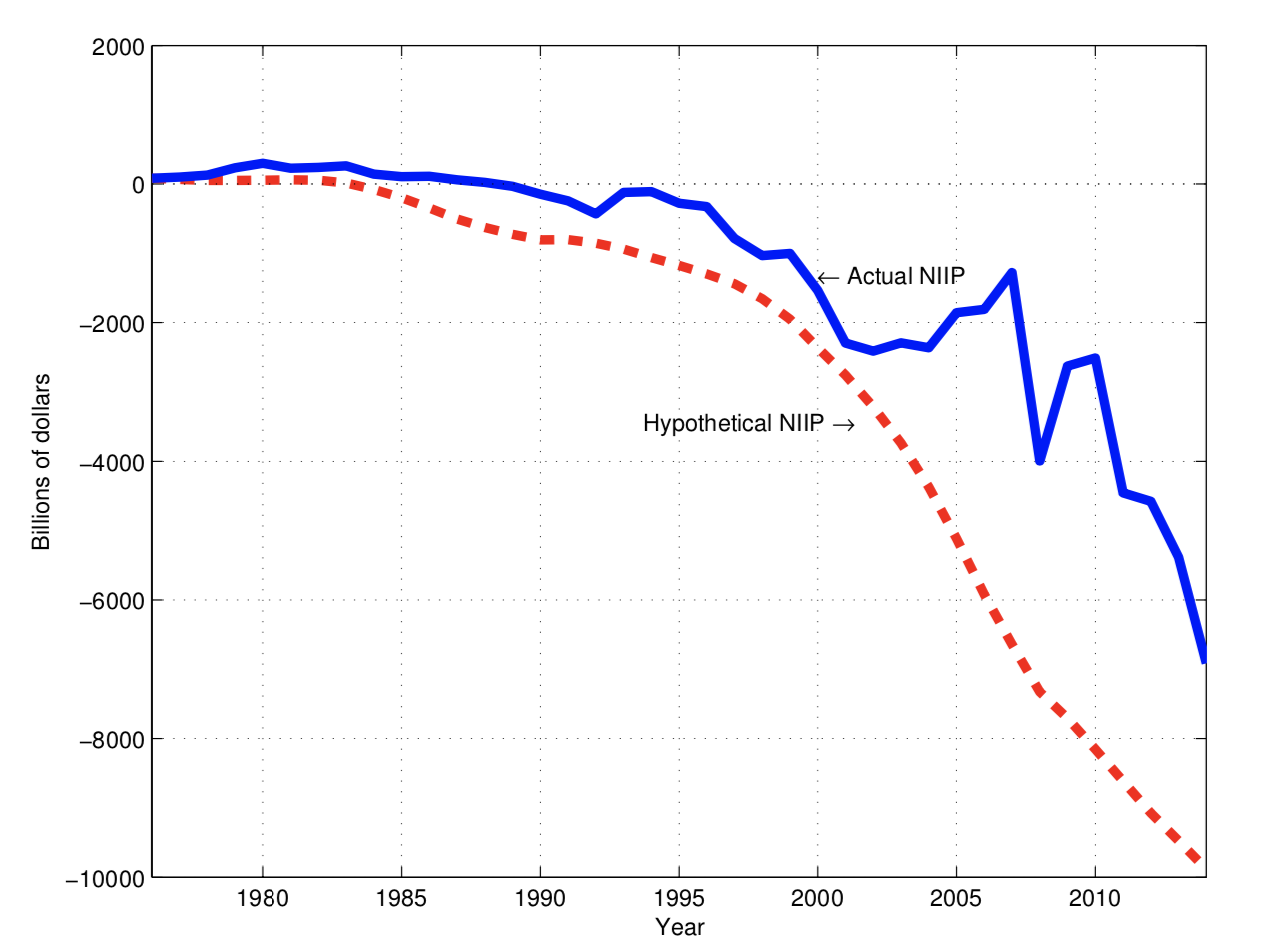
\includegraphics[width = 0.85\textwidth]{FIGURES/IIP_US.png}
%  \end{figure}
%  \vspace{-0.5cm}
%  \begin{minipage}{\columnwidth}
%  \footnotesize
%  Source: Schmitt-Grohe, Uribe, Woodford, Fig. 1.6.
%  \end{minipage}
%\end{frame}


\begin{frame}{Model for Balance of Payments and IIP}
  Recall the GDP decomposition (or desired demand equal to GDP): $Y_t = C_t + I_t + G_t + TB_t$ \vfill
  Consider a simple model with $I_t = 0, G_t = 0$, then: 
  \begin{align*}
  TB_t &= Y_t - C_t \\
  CA_t &= TB_t + r\cdot  IPP_t \\ &= \underbrace{Y_t+ r\cdot  IPP_t}_{\text{\tb{National Income}}} - C_t 
  \end{align*}
In this simple model, trade balance is difference of GDP and consumption, while current account is difference of National Income and consumption \\
\vfill
Can also use the formula in IIP dynamics:
 \begin{align*}
     IIP_{t+1} &= (1+r) IIP_t + TB_t \\
     \Leftrightarrow IIP_{t+1} &= (1+r) IIP_t + Y_t - C_t \\
 \end{align*}
\end{frame}

%  \begin{frame}{IIP and future trade balances}
%	\vspace{-5cm}
%	$$IIP_{t+1} = (1+r_t) IIP_t + TB_t $$
%	Recursive relationship. Substitute $IPP_{t+1}$, then $IPP_{t+2}$ and so on. Result?
%	
%
%  \end{frame}

%  \begin{frame}{IIP and future trade balances: interpretation}
%	\begin{mytemize}
%	  \item Assume $IIP_t<0$ -- country is a \textbf{net debtor} (not sovereign debt, but all sectors)
%	  \item Then, country must run future \tb{trade surplus} on average (with more importance to surpluses that are in near future)
%		\begin{mytemize}
%		\item Otherwise, debts cannot be repaid
%		\end{mytemize}
%	  \item Assume $IIP_t>0$ -- country is a \textbf{net creditor} of rest of the world 
%	  \item Then, country must run future \tb{trade deficits} on average (with more importance to deficits that are in near future)
%		\begin{mytemize}
%		\item Otherwise, debts of non-residents cannot be repaid
%		\end{mytemize}
%	\end{mytemize}
%	\vfill
%	\rarr Perpetual trade surpluses / trade deficits can be sustainable if very negative/very positive IIP to begin with. \textbf{$\{r_t\}$ matter, too}
%  \end{frame}
\section{Consumption in 2-period Open Economy}
\begin{frame}
\frametitle{Outline}
\tableofcontents[currentsection]
\end{frame}

\begin{frame}{A representative consumer}
    We now bring together the consumption problem and the BOP and IIP dynamics \\ \vfill
    Assume the GDP of the economy is an exogenous value perceived as income of \tb{representative consumer}
    \vfill
    The consumer has initial savings that correspond to the international investment position of the economy \\
    \vfill
    Studying consumption choices, we will determine trade balance and international investment position dynamics of the economy
\end{frame}
\begin{frame}{Resource constraint}
Since the representative consumer is only constrained by resources of the economy, we call her budget constraint the \tb{resource constraint}:
\begin{align*}
   IIP_{t+1} &= (1+r) IIP_t + Y_t - C_t \\
   IIP_{t+2} &= (1+r) IIP_{t+1} + Y_{t+1} - C_{t+1} 
\end{align*}

$IIP_{t+2} = 0$ as before, so inter-temporal resource constraint is obtained (by eliminating
\(IIP_{t+1}\)):
\[C_t + \frac{C_{t+1}}{1+ r} = (1+r)IIP_t + Y_t + \frac{Y_{t+1}}{1+r}\]
\vfill
 It can be used as a constraint in utility maximization of representative consumer
\end{frame}

\begin{frame}{2-period consumption in open economy: graph}
\vspace{-5cm} $IIP_{t+1}$ can be obtained as distance between $Y_t+(1+r)IIP_t$ and $C_t$
    
\end{frame}

%\begin{frame}{%
%\protect\hypertarget{productivity-shock-transitory-vs.permanent}{%
%Productivity shock: temporary vs.~permanent}}
%
%Assume a positive shock on period-1 productivity \(A_1\) \rarr GDP
%rises, but desired consumption also rises. What is the net effect on
%trade balance and current account?
%
%\begin{mytemize}
%
%\item
%  In this economy, net effect always \textbf{positive}: recall that
%  \(\Delta C_1 < \Delta Y_1\) because of consumption smoothing
%  \rarr \(\Delta TB_1 = \Delta Y_1 - \Delta C_1 > 0\). Same effect for
%  \(CA_1\) since \(CA_1 = TB_1 + r_1 \Omega_1\), with \(\Omega_1\)
%  pre-determined
%\item
%  The effect on \(TB_2\) must be negative, since
%  \(\Omega_1 = TB_1 + \frac{TB_2}{1+r_2}\) in a 2-period economy.
%  Another proof: \(\Delta C_2 > 0\) because of consumption smoothing,
%  but \(\Delta Y_2 = 0\).
%\end{mytemize}
%\vfill
%Then, assume a \textbf{permanent shock}: both \(A_1\) and \(A_2\) rise.
%What are effects on \(TB_1, CA_1\)?
%
%\begin{mytemize}
%
%\item
%  Ambiguous: the shock allows for \(\Delta C_1 > 0, \Delta C_2 > 0\)
%  with both \(\Delta C_1> \Delta Y_1\) and \(\Delta C_1< \Delta Y_1\).
%\end{mytemize}
%
%\end{frame}


\end{document}
